% Figure from MATH 591 notes, section 16. Compile with the notes preamble.
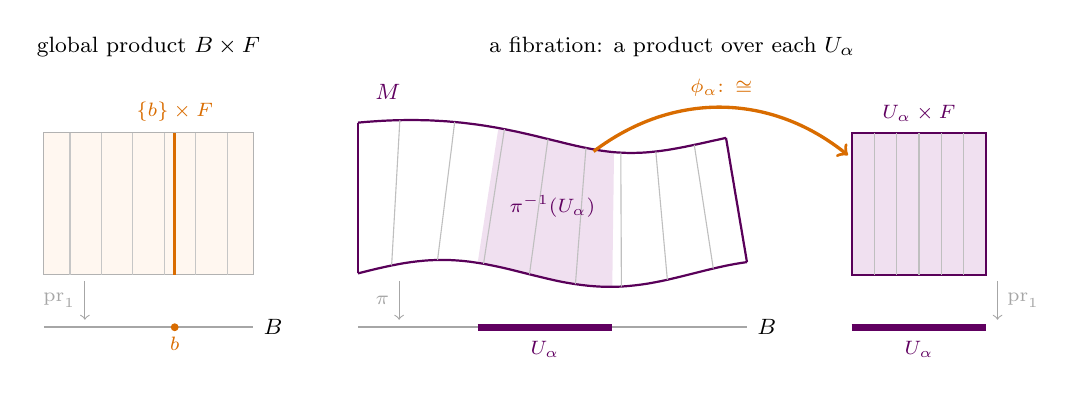
\begin{tikzpicture}[scale=0.95]
\fill[orange!6] (0,0.7) rectangle (2.8,2.6); \draw[gray!60] (0,0.7) rectangle (2.8,2.6);
\draw[gray!45] (0.35,0.7) -- (0.35,2.6);
\draw[gray!45] (0.77,0.7) -- (0.77,2.6);
\draw[gray!45] (1.19,0.7) -- (1.19,2.6);
\draw[gray!45] (1.61,0.7) -- (1.61,2.6);
\draw[gray!45] (2.03,0.7) -- (2.03,2.6);
\draw[gray!45] (2.45,0.7) -- (2.45,2.6);
\draw[orange!85!black, very thick] (1.75,0.7) -- (1.75,2.6); \node[orange!85!black, font=\scriptsize, anchor=south] at (1.75,2.62) {$\{b\} \times F$};
\draw[thick, gray!70] (0,0) -- (2.8,0) node[right, font=\footnotesize, text=black] {$B$}; \fill[orange!85!black] (1.75,0) circle (1.5pt) node[below, font=\scriptsize] {$b$};
\draw[->, gray!70] (0.55,0.62) -- node[left, font=\scriptsize] {$\mathrm{pr}_1$} (0.55,0.1);
\node[font=\footnotesize] at (1.4,3.75) {global product $B \times F$};
\fill[violet!12] (5.800,0.861) -- (5.825,1.025) -- (5.850,1.189) -- (5.876,1.353) -- (5.901,1.517) -- (5.926,1.680) -- (5.951,1.844) -- (5.977,2.008) -- (6.002,2.172) -- (6.027,2.336) -- (6.052,2.500) -- (6.078,2.663) -- (6.078,2.663) -- (6.174,2.645) -- (6.269,2.626) -- (6.362,2.606) -- (6.453,2.586) -- (6.542,2.565) -- (6.628,2.544) -- (6.713,2.523) -- (6.796,2.503) -- (6.878,2.483) -- (6.958,2.463) -- (7.036,2.444) -- (7.113,2.427) -- (7.188,2.410) -- (7.262,2.395) -- (7.336,2.381) -- (7.408,2.368) -- (7.480,2.357) -- (7.552,2.348) -- (7.623,2.341) -- (7.623,2.341) -- (7.621,2.177) -- (7.619,2.013) -- (7.617,1.850) -- (7.615,1.686) -- (7.612,1.522) -- (7.610,1.359) -- (7.608,1.195) -- (7.606,1.031) -- (7.604,0.868) -- (7.602,0.704) -- (7.600,0.540) -- (7.600,0.540) -- (7.505,0.541) -- (7.411,0.544) -- (7.316,0.551) -- (7.221,0.561) -- (7.126,0.573) -- (7.032,0.588) -- (6.937,0.605) -- (6.842,0.625) -- (6.747,0.646) -- (6.653,0.668) -- (6.558,0.691) -- (6.463,0.715) -- (6.368,0.739) -- (6.274,0.763) -- (6.179,0.785) -- (6.084,0.807) -- (5.989,0.827) -- (5.895,0.845) -- (5.800,0.861) -- cycle;
\draw[violet!70!black, thick] (4.200,0.720) -- (4.288,0.742) -- (4.376,0.764) -- (4.464,0.785) -- (4.553,0.805) -- (4.641,0.824) -- (4.729,0.841) -- (4.817,0.857) -- (4.905,0.870) -- (4.993,0.881) -- (5.081,0.890) -- (5.169,0.896) -- (5.258,0.899) -- (5.346,0.900) -- (5.434,0.898) -- (5.522,0.893) -- (5.610,0.886) -- (5.698,0.876) -- (5.786,0.863) -- (5.875,0.849) -- (5.963,0.832) -- (6.051,0.814) -- (6.139,0.795) -- (6.227,0.774) -- (6.315,0.752) -- (6.403,0.730) -- (6.492,0.708) -- (6.580,0.686) -- (6.668,0.665) -- (6.756,0.644) -- (6.844,0.624) -- (6.932,0.606) -- (7.020,0.590) -- (7.108,0.576) -- (7.197,0.564) -- (7.285,0.554) -- (7.373,0.547) -- (7.461,0.542) -- (7.549,0.540) -- (7.637,0.541) -- (7.725,0.544) -- (7.814,0.551) -- (7.902,0.560) -- (7.990,0.571) -- (8.078,0.584) -- (8.166,0.600) -- (8.254,0.617) -- (8.342,0.636) -- (8.431,0.657) -- (8.519,0.678) -- (8.607,0.700) -- (8.695,0.722) -- (8.783,0.744) -- (8.871,0.766) -- (8.959,0.787) -- (9.047,0.807) -- (9.136,0.826) -- (9.224,0.843) -- (9.312,0.858) -- (9.400,0.871); \draw[violet!70!black, thick] (4.200,2.735) -- (4.310,2.745) -- (4.421,2.753) -- (4.530,2.760) -- (4.640,2.765) -- (4.749,2.768) -- (4.857,2.770) -- (4.965,2.770) -- (5.071,2.768) -- (5.177,2.765) -- (5.281,2.759) -- (5.384,2.753) -- (5.486,2.744) -- (5.586,2.735) -- (5.685,2.723) -- (5.782,2.711) -- (5.878,2.697) -- (5.971,2.682) -- (6.064,2.666) -- (6.154,2.649) -- (6.243,2.631) -- (6.330,2.613) -- (6.415,2.594) -- (6.498,2.575) -- (6.580,2.556) -- (6.660,2.536) -- (6.738,2.517) -- (6.815,2.498) -- (6.891,2.480) -- (6.965,2.461) -- (7.037,2.444) -- (7.109,2.427) -- (7.179,2.412) -- (7.249,2.397) -- (7.317,2.384) -- (7.385,2.372) -- (7.452,2.361) -- (7.518,2.352) -- (7.585,2.344) -- (7.651,2.338) -- (7.717,2.334) -- (7.783,2.331) -- (7.849,2.330) -- (7.915,2.331) -- (7.982,2.333) -- (8.050,2.337) -- (8.118,2.343) -- (8.187,2.350) -- (8.258,2.359) -- (8.329,2.369) -- (8.401,2.381) -- (8.475,2.394) -- (8.550,2.408) -- (8.627,2.424) -- (8.705,2.440) -- (8.784,2.457) -- (8.866,2.475) -- (8.949,2.494) -- (9.034,2.512) -- (9.120,2.532);
\draw[violet!70!black, thick] (4.200,0.720) -- (4.200,0.903) -- (4.200,1.086) -- (4.200,1.270) -- (4.200,1.453) -- (4.200,1.636) -- (4.200,1.819) -- (4.200,2.002) -- (4.200,2.186) -- (4.200,2.369) -- (4.200,2.552) -- (4.200,2.735); \draw[violet!70!black, thick] (9.400,0.871) -- (9.375,1.022) -- (9.349,1.173) -- (9.324,1.324) -- (9.298,1.475) -- (9.273,1.626) -- (9.247,1.777) -- (9.222,1.928) -- (9.196,2.079) -- (9.171,2.230) -- (9.146,2.381) -- (9.120,2.532);
\draw[gray!50] (4.650,0.826) -- (4.660,1.003) -- (4.670,1.179) -- (4.680,1.356) -- (4.690,1.532) -- (4.700,1.709) -- (4.710,1.886) -- (4.720,2.062) -- (4.730,2.239) -- (4.740,2.415) -- (4.750,2.592) -- (4.760,2.768);
\draw[gray!50] (5.264,0.899) -- (5.285,1.067) -- (5.306,1.235) -- (5.327,1.402) -- (5.348,1.570) -- (5.368,1.738) -- (5.389,1.905) -- (5.410,2.073) -- (5.431,2.241) -- (5.452,2.408) -- (5.472,2.576) -- (5.493,2.744);
\draw[gray!50] (5.879,0.848) -- (5.904,1.012) -- (5.929,1.175) -- (5.955,1.339) -- (5.980,1.503) -- (6.006,1.666) -- (6.031,1.830) -- (6.056,1.994) -- (6.082,2.157) -- (6.107,2.321) -- (6.133,2.485) -- (6.158,2.648);
\draw[gray!50] (6.493,0.708) -- (6.515,0.872) -- (6.538,1.037) -- (6.560,1.201) -- (6.583,1.366) -- (6.605,1.530) -- (6.627,1.695) -- (6.650,1.859) -- (6.672,2.023) -- (6.695,2.188) -- (6.717,2.352) -- (6.740,2.517);
\draw[gray!50] (7.107,0.576) -- (7.120,0.741) -- (7.133,0.907) -- (7.145,1.073) -- (7.158,1.238) -- (7.171,1.404) -- (7.184,1.570) -- (7.196,1.735) -- (7.209,1.901) -- (7.222,2.066) -- (7.235,2.232) -- (7.248,2.398);
\draw[gray!50] (7.721,0.544) -- (7.721,0.707) -- (7.720,0.870) -- (7.719,1.032) -- (7.719,1.195) -- (7.718,1.358) -- (7.717,1.520) -- (7.716,1.683) -- (7.716,1.846) -- (7.715,2.009) -- (7.714,2.171) -- (7.714,2.334);
\draw[gray!50] (8.336,0.635) -- (8.322,0.791) -- (8.308,0.947) -- (8.294,1.102) -- (8.280,1.258) -- (8.266,1.414) -- (8.252,1.570) -- (8.238,1.726) -- (8.224,1.882) -- (8.210,2.038) -- (8.196,2.194) -- (8.182,2.349);
\draw[gray!50] (8.950,0.785) -- (8.927,0.935) -- (8.904,1.085) -- (8.881,1.236) -- (8.858,1.386) -- (8.835,1.536) -- (8.812,1.687) -- (8.789,1.837) -- (8.766,1.987) -- (8.742,2.138) -- (8.719,2.288) -- (8.696,2.438);
\node[violet!75!black, font=\footnotesize] at (4.60,3.15) {$M$};
\node[violet!75!black, font=\scriptsize] at (6.80,1.62) {$\pi^{-1}(U_\alpha)$};
\draw[thick, gray!70] (4.20,0) -- (9.40,0) node[right, font=\footnotesize, text=black] {$B$};
\draw[violet!75!black, line width=2.4pt] (5.80,0) -- (7.60,0); \node[violet!75!black, font=\scriptsize] at (6.70,-0.3) {$U_\alpha$};
\draw[->, gray!70] (4.75,0.62) -- node[left, font=\scriptsize] {$\pi$} (4.75,0.1);
\fill[violet!12] (10.80,0.7) rectangle (12.60,2.6); \draw[violet!70!black, thick] (10.80,0.7) rectangle (12.60,2.6);
\draw[gray!50] (11.10,0.7) -- (11.10,2.6);
\draw[gray!50] (11.40,0.7) -- (11.40,2.6);
\draw[gray!50] (11.70,0.7) -- (11.70,2.6);
\draw[gray!50] (12.00,0.7) -- (12.00,2.6);
\draw[gray!50] (12.30,0.7) -- (12.30,2.6);
\node[violet!75!black, font=\scriptsize, anchor=south] at (11.70,2.62) {$U_\alpha \times F$};
\draw[violet!75!black, line width=2.4pt] (10.80,0) -- (12.60,0); \node[violet!75!black, font=\scriptsize] at (11.70,-0.3) {$U_\alpha$};
\draw[->, gray!70] (12.75,0.62) -- node[right, font=\scriptsize] {$\mathrm{pr}_1$} (12.75,0.1);
\draw[->, very thick, orange!85!black] (7.35,2.35) to[bend left=38] node[above, font=\scriptsize] {$\phi_\alpha \colon\ \cong$} (10.75,2.3);
\node[font=\footnotesize] at (8.40,3.75) {a fibration: a product over each $U_\alpha$};
\end{tikzpicture}
